\begin{figure}[htbp]
  \centering
  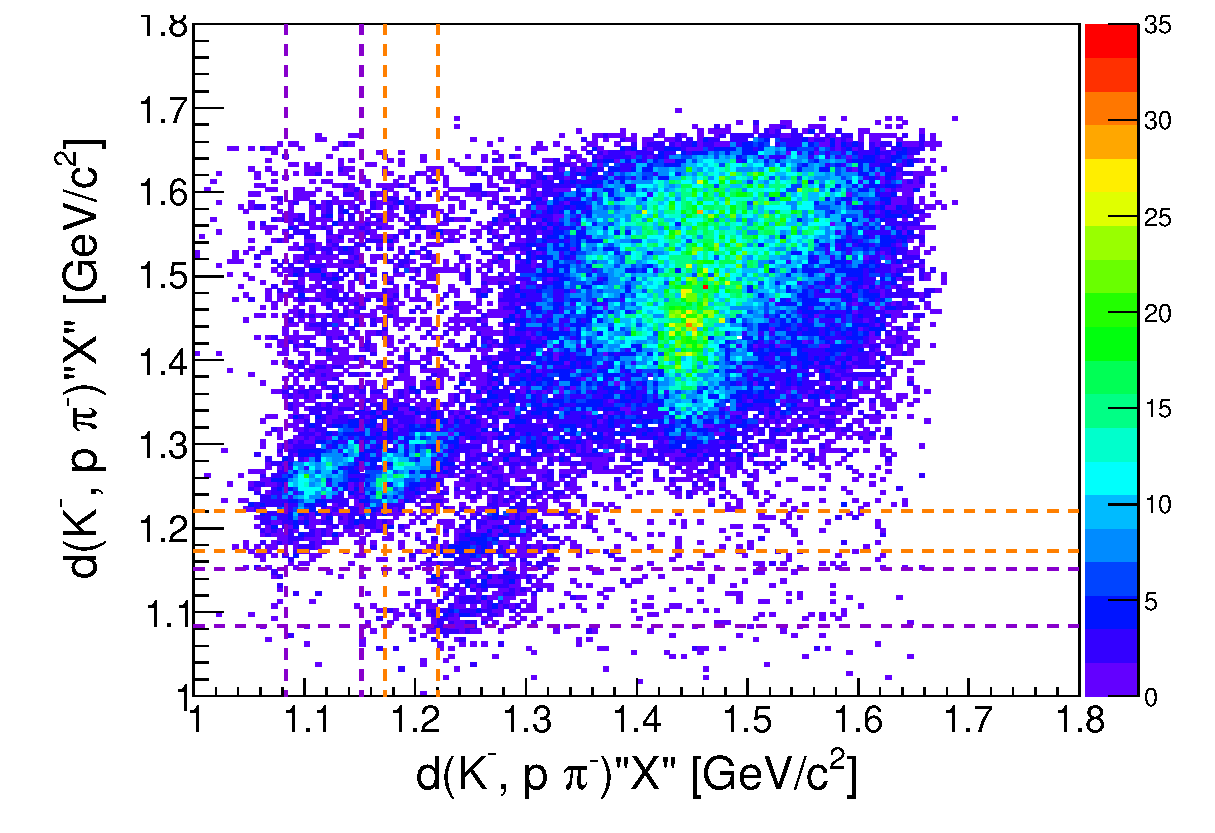
\includegraphics[width=8cm]{../pic/Run68/KP_ana/KPpim_KPpim_MM.eps}
  \caption{
    This figure shows the scatter plot of the $d(K^-, p \pi^-)$ missing masses in the $p$ and two $\pi^-$ detected events.
    Horizontal axis represents nearer DCA $\pi^-$ and virtical axis represents other one.
    Orange and purple lines indicate selection region as $d(K^-, p \pi^-)"\Sigma^0"$ and $d(K^-, p \pi^-)"\Lambda"$, respectively.
  }
  \label{fig:KPpim_KPpim}
\end{figure}
